% ----------------------------------------------------------
% Introdução
% ----------------------------------------------------------
\chapter{Introdução}\label{ch:intro}
Aqui vai o texto da introdução.

A ABNT indica a elaboração de uma lista de ilustrações com todos os itens arrolados e designados por seu nome específico, conforme a ordem que aparecem no texto (Figura 1, Fotografia 1, Gráfico 1, Quadro 1, entre outros). Também recomenda, quando necessário, a elaboração de lista própria para cada tipo de ilustração. No entanto, não determina um número mínimo de ilustrações para tal lista específica.

\section{Tema}\label{sec:tema}

escreva aqui...

\subsection{Delimitação do tema}\label{sec:deltema}
Aqui vai a delimitação do tema se tiver descrito na seção~\ref{sec:tema}.




\section{Problema}\label{sec:probPesquisa}
escreva aqui...

\section{Objetivo geral}\label{sec:objGeral}
escreva aqui...

\subsection{Objetivos Específicos}\label{sec:objEsp}
\begin{enumerate}
	\item objetivo especifico aqui...
	\item objetivo especifico aqui...
\end{enumerate}

\section{Justificativa}\label{sec:just}
escreva aqui...

\chapter{Referencial Teórico}\label{ch:ref}
aqui vai o texto do referencial teórico. 

Vc deve inserir novas seções e subseções. Recomendo usar labels para todas as seções.

\section{Citações}\label{sec:citacao}

Este parágrafo serve apenas para explicar as citações de referências. 

Os dois parágrafos a seguir mostram, respectivamente, como fazer uma citação indireta e direta. 

Conforme~\citeauthoronline{bourg2013physics}, o quadrado não é redondo e o círculo não é quadrado. Esta próxima citação é do tipo direta, onde copiamos uma frase inteira do autor. 

Poderíamos refletir sobre a "existência de quadrados redondos e círculos quadrados"~\cite{ericson2004real}. 


\subsection{Citação longa}\label{subsec:citacaoLonga}

O texto abaixo demonstra uma citação direta com mais de 3 linhas. Segundo~\cite{ericson2004real}:

\begin{citacao}
	O texto deve ser constituído de uma parte introdutória, na qual devem ser
	expostos o tema do projeto, o problema a ser abordado, a(s) hipótese(s),
	quando couber(em), bem como o(s) objetivo(s) a ser(em) atingido(s) e a(s)
	justificativa(s). É necessário que sejam indicados o referencial teórico que
	o embasa, a metodologia a ser utilizada, assim como os recursos e o cronograma
	necessários à sua consecução.
\end{citacao}


\section{Uso de quadros para códigos}\label{sec:quadros}

Quadro é um espaço não afetado pelas formatações do latex. O quadro aceita apenas texto em UTF-8 (textos com caracteres especias precisam de outra solução).

A referencia~\cite{ericson2004real} é retirada de um livro, enquanto a referência~\cite{Silverman20201569} é de um artigo. O tipo de publicação é informado no arquivo \emph{bibliografia.bib}. 

O quadro~\ref{lst:quadro1} mostra um exemplo de referencia armazenada no arquivo das \emph{bibliografia.bib}.

\begin{lstlisting}[caption={Exemplo referência},label={lst:quadro1}]
@ARTICLE{Silverman20201569,
	author = {Silverman, Linda K. and Gilman, Barbara J.},
	title = {Best practices in gifted identification and assessment: 
		Lessons from the WISC-V},
	year = {2020},
	journal = {Psychology in the Schools},
	volume = {57},
	number = {10},
	pages = {}1569 - 1581},
	doi = {10.1002/pits.22361},
	url = {https:/link.com.br},
	type = {Article},
	publication_stage = {Final},
	source = {Scopus},
	note = {Cited by: 14}
}
\end{lstlisting}
	

\section{Ilustrações}\label{sec:ilustrações}
Este parágrafo serve apenas para explicar como é inserido uma imagem. Não devem existir figuras não referenciadas no corpo do texto. A Figura~\ref{fig:figura1} mostra duas formas geométricas, enquanto a Figura~\ref{fig:figura2} mostra o diagrama de uma arquitetura imaginária de autoria própria.

\begin{figure}[htb]
	\centering
	\caption{\label{fig:figura1} Figura apresentando uma representação gráfica de uma esfera a esquerda e um cubo a direita.}
	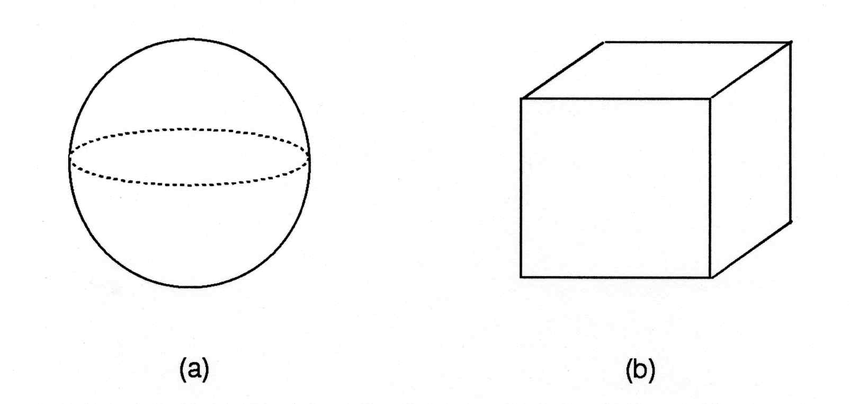
\includegraphics[width=\textwidth]{imgs/figura1.png}
	\legend{Fonte: \cite{bourg2013physics}.}
\end{figure}

No campo $\backslash$caption vai a label da figura (que é única em todo texto ) e a descrição da figura (chamamos de legenda). No campo $\backslash$legenda vai a fonte, informando a origem da figura. A instrução $\backslash$centering faz com que os elementos sejam centralizados.


\begin{figure}[htb]
	\centering
	\caption{\label{fig:figura2} Arquitetura imprevista: um sistema projetado para um projeto de pesquisa que pesquisaria algo.}
	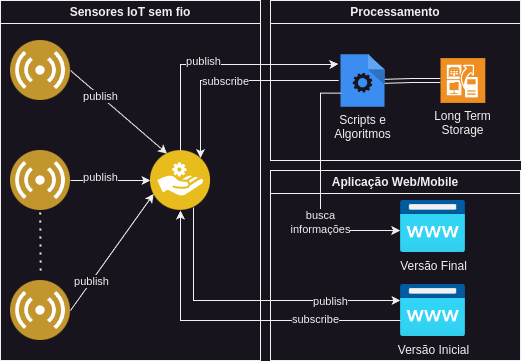
\includegraphics[scale=0.5]{imgs/arquitetura.png}
	\legend{Fonte: Do autor (2024). }
\end{figure}

Observe a diferença do comando $\backslash$includegraphics nas figuras. Na Figura~\ref{fig:figura1} a imagem é configurada para ocupar toda largura da página, enquanto a Figura~\ref{fig:figura2} trabalha escala. Se escala = 1 a figura é mostrada no tamanho original, se escala = 0.5 a figura é mostrada com 50\% do seu tamanho. 

\section{Trabalhos relacionados}

O Código~\ref{lst:quadro2} apresenta um trecho de código mágico, escrito na linguagem C++.

\begin{lstlisting}[caption={Exemplo de laço},label={lst:quadro2}]
	void func(int){
	for(int =0;i<10;i++){
		fprintf("asdfas fddfsadf");
	
		}
	}
\end{lstlisting}


\chapter{Metodologia}
escreva aqui...

\section{Arquitetura}
escreva aqui...

\section{Recursos}
escreva aqui...

\subsection{Cronograma}
escreva aqui...

As ações necessárias para a execução do projeto são:
\begin{enumerate}
	\item A tabela a seguir é organizada de forma quinzenal;
	\item Recomendo criar uma lista de atividades e apenas referenciar na tabela;
	\item Esta lista pode ser usada para Nomear e explicar as atividades (ações) do projeto;
	\item ....
	\item ....
	\item ....
	\item Apresentação do projeto à banca avaliadora.
\end{enumerate}

O Quadro~\ref{cronograma} apresenta a distribuição das atividades planejadas em um cronograma semanal. Para editar no modo latex, recomendo remover a quebra de linha no editor usado ou então montar a tabela em um gerador de tabela em Latex. Veja em $https://www.tablesgenerator.com/latex_tables$

Para utilizar as instruções pré-prontas, basta marcar com X no quadrinho desejado. Por exemplo, vamos definir que a atividade 1 será executada em Fevereiro, nas semanas 1 e 2. Para tanto, marcamos x no \verb*|{}| vazio, ficando assim 
\begin{verbatim}
	1	& \multicolumn{1}{c|}{x} & \multicolumn{1}{c|}{x} & \multicolumn{1}{c|}{}....
\end{verbatim}




\begin{quadro}[htb]
\smaller
\caption{\label{cronograma}Quadro apresentando o cronograma semanal previsto.}	
\begin{tabular}{|c|cccc|cccc|cccc|cccc|cccc|cccc|}
\rowcolor{gray}
%linha dos meses: alterar os meses se necessário  
	& \multicolumn{4}{c|}{\textbf{Fevereiro}} & \multicolumn{4}{c|}{\textbf{Março}} & \multicolumn{4}{|c|}{\textbf{Abril}} & \multicolumn{4}{c|}{\textbf{Maio}} & \multicolumn{4}{c}{\textbf{Junho}} & \multicolumn{4}{c}{\textbf{Julho}} \\
%linha das semanas (cada mes tem 4 semanas)
AÇÃO	& \multicolumn{1}{c|}{1} & \multicolumn{1}{c|}{2} & \multicolumn{1}{c|}{3} & 4 & \multicolumn{1}{c|}{1} & \multicolumn{1}{c|}{2} & \multicolumn{1}{c|}{3} & 4 & \multicolumn{1}{c|}{1} & \multicolumn{1}{c|}{2} & \multicolumn{1}{c|}{3} & 4 & \multicolumn{1}{c|}{1} & \multicolumn{1}{c|}{2} & \multicolumn{1}{c|}{3} & 4 & \multicolumn{1}{c|}{1} & \multicolumn{1}{c|}{2} & \multicolumn{1}{c|}{3} & 4 & \multicolumn{1}{c|}{1} & \multicolumn{1}{c|}{2} & \multicolumn{1}{c|}{3} & 4 \\ \hline
%linhas das atividades: Marcar X na semana em que a ação será desenvolvida	
1	& \multicolumn{1}{c|}{x} & \multicolumn{1}{c|}{x} & \multicolumn{1}{c|}{}  &   & \multicolumn{1}{c|}{}  & \multicolumn{1}{c|}{}  & \multicolumn{1}{c|}{}  &   & \multicolumn{1}{c|}{}  & \multicolumn{1}{c|}{}  & \multicolumn{1}{c|}{}  &   & \multicolumn{1}{c|}{}  & \multicolumn{1}{c|}{}  & \multicolumn{1}{c|}{}  &   & \multicolumn{1}{c|}{}  & \multicolumn{1}{c|}{}  & \multicolumn{1}{c|}{}  &   & \multicolumn{1}{c|}{}  & \multicolumn{1}{c|}{}  & \multicolumn{1}{c|}{}  &   \\ \hline

2 	& \multicolumn{1}{c|}{} & \multicolumn{1}{c|}{} & \multicolumn{1}{c|}{}  &   & \multicolumn{1}{c|}{}  & \multicolumn{1}{c|}{}  & \multicolumn{1}{c|}{}  &   & \multicolumn{1}{c|}{}  & \multicolumn{1}{c|}{}  & \multicolumn{1}{c|}{}  &   & \multicolumn{1}{c|}{}  & \multicolumn{1}{c|}{}  & \multicolumn{1}{c|}{}  &   & \multicolumn{1}{c|}{}  & \multicolumn{1}{c|}{}  & \multicolumn{1}{c|}{}  &   & \multicolumn{1}{c|}{}  & \multicolumn{1}{c|}{}  & \multicolumn{1}{c|}{}  &   \\ \hline

3 	& \multicolumn{1}{c|}{} & \multicolumn{1}{c|}{} & \multicolumn{1}{c|}{}  &   & \multicolumn{1}{c|}{}  & \multicolumn{1}{c|}{}  & \multicolumn{1}{c|}{}  &   & \multicolumn{1}{c|}{}  & \multicolumn{1}{c|}{}  & \multicolumn{1}{c|}{}  &   & \multicolumn{1}{c|}{}  & \multicolumn{1}{c|}{}  & \multicolumn{1}{c|}{}  &   & \multicolumn{1}{c|}{}  & \multicolumn{1}{c|}{}  & \multicolumn{1}{c|}{}  &   & \multicolumn{1}{c|}{}  & \multicolumn{1}{c|}{}  & \multicolumn{1}{c|}{}  &   \\ \hline

4 	& \multicolumn{1}{c|}{} & \multicolumn{1}{c|}{} & \multicolumn{1}{c|}{}  &   & \multicolumn{1}{c|}{}  & \multicolumn{1}{c|}{}  & \multicolumn{1}{c|}{}  &   & \multicolumn{1}{c|}{}  & \multicolumn{1}{c|}{}  & \multicolumn{1}{c|}{}  &   & \multicolumn{1}{c|}{}  & \multicolumn{1}{c|}{}  & \multicolumn{1}{c|}{}  &   & \multicolumn{1}{c|}{}  & \multicolumn{1}{c|}{}  & \multicolumn{1}{c|}{}  &   & \multicolumn{1}{c|}{}  & \multicolumn{1}{c|}{}  & \multicolumn{1}{c|}{}  &   \\ \hline

6 	& \multicolumn{1}{c|}{} & \multicolumn{1}{c|}{} & \multicolumn{1}{c|}{}  &   & \multicolumn{1}{c|}{}  & \multicolumn{1}{c|}{}  & \multicolumn{1}{c|}{}  &   & \multicolumn{1}{c|}{}  & \multicolumn{1}{c|}{}  & \multicolumn{1}{c|}{}  &   & \multicolumn{1}{c|}{}  & \multicolumn{1}{c|}{}  & \multicolumn{1}{c|}{}  &   & \multicolumn{1}{c|}{}  & \multicolumn{1}{c|}{}  & \multicolumn{1}{c|}{}  &   & \multicolumn{1}{c|}{}  & \multicolumn{1}{c|}{}  & \multicolumn{1}{c|}{}  &   \\ \hline

7 	& \multicolumn{1}{c|}{} & \multicolumn{1}{c|}{} & \multicolumn{1}{c|}{}  &   & \multicolumn{1}{c|}{}  & \multicolumn{1}{c|}{}  & \multicolumn{1}{c|}{}  &   & \multicolumn{1}{c|}{}  & \multicolumn{1}{c|}{}  & \multicolumn{1}{c|}{}  &   & \multicolumn{1}{c|}{}  & \multicolumn{1}{c|}{}  & \multicolumn{1}{c|}{}  &   & \multicolumn{1}{c|}{}  & \multicolumn{1}{c|}{}  & \multicolumn{1}{c|}{}  &   & \multicolumn{1}{c|}{}  & \multicolumn{1}{c|}{}  & \multicolumn{1}{c|}{}  &   \\ \hline

\end{tabular}
\end{quadro}
